\documentclass[tikz]{standalone}
\usepackage{ctex}
\usepackage{tikz}
\usepackage{pgfplots}
\pgfplotsset{compat=1.18}   % 使用较新版本语法
\usetikzlibrary{positioning, arrows.meta, intersections, calc, fit, backgrounds}
\usepgfplotslibrary{fillbetween}  % 用于填充区域

\begin{document}
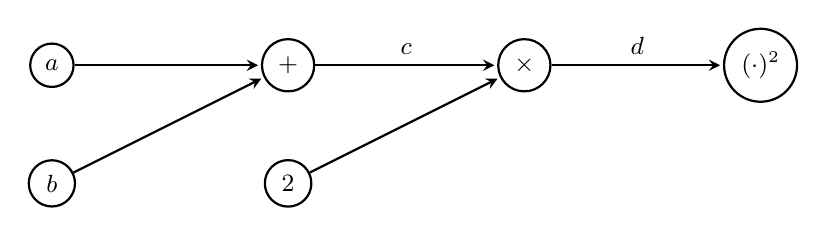
\begin{tikzpicture}[->,>=stealth,shorten >=1pt,auto,node distance=1.5cm,
    thick,main node/.style={circle,draw,font=\sffamily\small}]
    \node[main node] (a) {$a$};
    \node[main node] (b) [below of=a] {$b$};
    \node[main node] (c) [right of=a, xshift=1.5cm] {$+$};
    \node[main node] (two) [below of=c] {$2$};
    \node[main node] (d) [right of=c, xshift=1.5cm] {$\times$};
    \node[main node] (L) [right of=d, xshift=1.5cm] {$(\cdot)^2$};
    \path[every node/.style={font=\sffamily\small}]
    (a) edge node {} (c)
    (b) edge node {} (c)
    (c) edge node {$c$} (d)
    (two) edge node {} (d)
    (d) edge node {$d$} (L);
\end{tikzpicture}

\end{document}
